% LaTeX template for Finance summaries
% Stu Alden
%-----------------------------------------
% Compount Interest I
% Basic Compound Interest Notes

\documentclass[14pt]{extarticle}

\usepackage{finmath}


%---------------------------------------
\begin{document}

\finmathtitle{Compound Interest I}

\textbf{Compound Interest} is just geometric or exponential growth
of money.  The compound interest rate is the rate of growth over a period
of time, as a percentage of the amount at the \underline{beginning} of the period.

The period is sometimes called an interest \textbf{conversion} period. It's called \underline{compound}
interest because each period's interest is based on \underline{all} past amounts including past interest.  So
if we use the following notation:
\begin{center}
    \renewcommand{\arraystretch}{1.2}
    \begin{tabular}{rl}
        \textbf{A} & Starting amount (Present Value or PV)           \\
        \textbf{S} & Final amount (Future Value or FV)               \\
        \textbf{i} & Interest rate per period (as a decimal, \%/100) \\
        \textbf{n} & Number of periods (can be fractional)
    \end{tabular}
\end{center}

After one period:
\[
    A \rightarrow A(1+i)
\]

After two periods:
\[
    A(1+i) \rightarrow A(1+i)^2
\]

Repeating this process for $n$ periods gives

\[
    S = A(1+i)^n
\]

Conversely,

\[
    A = \frac{S}{(1+i)^n}
    = S(1+i)^{-n}
    = Sv^n
\]

where

\[
    v = \frac{1}{1+i} = (1+i)^{-1}
\]


\newpage
A timeline looks like this:

\begin{center}
    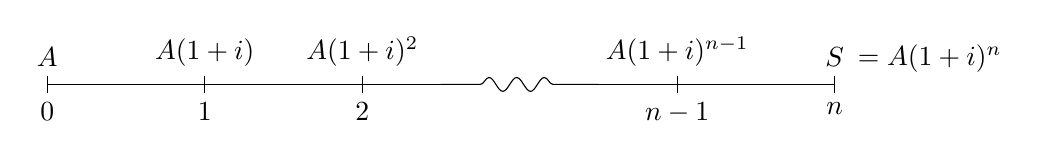
\begin{tikzpicture}
        %draw horizontal line with squiggle in middle
        \draw (0,0) -- (5,0);
        \draw[decorate,decoration={snake,pre length=5mm, post length=5mm}] (5,0) -- (7,0);
        \draw (7,0) -- (10,0);

        %draw vertical tick-marks
        \foreach \x in {0,2,4,8,10}
        \draw (\x cm,3pt) -- (\x cm,-3pt);

        %Label "nodes"
        \draw (0,0) node[below=3pt] {$ 0 $} node[above=3pt] {$ A $};

        \draw (2,0) node[below=3pt] {$ 1 $} node[above=3pt] {$ A(1+i) $};

        \draw (4,0) node[below=3pt] {$ 2 $} node[above=3pt] {$ A(1+i)^2 $};

        \draw (6,0) node[below=3pt] {$  $} node[above=3pt] {$  $};

        \draw (8,0) node[below=3pt] {$ n - 1 $} node[above=3pt] {$ A(1+i)^{n-1} $};

        \draw (10,0) node[below=3pt] {$ n $}
        node[above=3pt] (Sn) {$ S $};

        \draw (Sn.north east)
        node[anchor=north west, xshift=-0.2em, yshift=0.25ex]
        {$=A(1+i)^n$};

    \end{tikzpicture}
\end{center}

\smallskip
\textbf{Notes:}

\begin{itemize}
    \item Multiplying by the factor $ (1+i)^t $ (> 1.0, growing) is called \textbf{``accumulating t periods.''}
    \item Multiplying by the factor $ v^t $ (< 1.0, shrinking) is called \textbf{``discounting t periods.''}
    \item Knowing any three of the variables $A$, $S$, $n$ and $i$, you can solve for the fourth.
    \item For anything beyond the simplest problems, drawing a timeline (even if just ``in your head'')
          is \underline{essential}!  It's the only way to ensure that your equation is correct.
\end{itemize}

\end{document}
